\documentclass[10pt, a4paper]{article}

\usepackage[paper=a4paper, left=1.5cm, right=1.5cm, bottom=1.5cm, top=1.5cm]{geometry}
\usepackage[utf8]{inputenc}
\usepackage[spanish]{babel}
\usepackage{graphicx}
\usepackage{multicol}
\usepackage[usenames,dvipsnames]{color}
\usepackage{amsmath}
\usepackage{verbatim}
\usepackage{footnote}
\usepackage{float}
\usepackage{amsfonts}
\usepackage{hyperref}
\usepackage{framed}
\usepackage{pdflscape}

\usepackage{pdfpages}

\usepackage{caratula}


\materia{Ingeniería de Software II}

\titulo{Trabajo Práctico 1}
\subtitulo{Sprint Planning}

\integrante{Martín Alejandro Miguel}{181/09}{m2.march@gmail.com}
\integrante{Iván Postolski}{216/09}{ivan.postolski@gmail.com}
\integrante{Juan Manuel Martinez Caamaño}{276/09}{jmartinezcaamao@gmail.com}
\integrante{Matías Incem}{396/09}{matias.incem@gmail.com}
\integrante{Pablo Gauna}{334/09}{gaunapablo@gmail.com}


\begin{document}

\maketitle
\tableofcontents
\newpage

\section{Introducción}

El actual informe presenta el análisis, diseño y desarrollo inicial realizado para el producto \textbf{Precio Justo}. En el mismo se detallan el conjunto de \emph{user stories} que abarcan el desarrollo completo de la aplicación, incluyendo tanto las definiciones actuales como los puntos de extensión que se tendrán en cuenta. Se presenta además un primer \emph{diseño orientado a objetos} de la aplicación completa. Este tiene como intención estar abierto a los distintos ejes de cambios considerados en esta instancia. Por último, se analiza el alcance, el proceso y el éxito de la primera iteración del proceso de desarrollo. En esta sección se explica lo logrado y se generan conclusiones y propuestas de cambio para el resto del proceso.

\section{Análisis de la aplicación}

\subsection{Objetivo}

\textbf{Precio Justo} es una aplicación de recolección y procesamiento de datos masivos provistos por redes sociales. La intención es poder recopilar los precios más baratos para ciertos productos, de forma confiable y libre de intereses particulares. La elección del uso de las redes sociales para obtener los datos tiene como objetivo lograr imparcialidad en los mismos.

\subsection{Ejes de cambio}

Dentro de la resolución del objetivo de la aplicación se establecen, para una primera instancia, las siguientes restricciones, que pasan a conformar \emph{ejes de cambio} de la aplicación:

\paragraph{Obtención de datos}
\begin{itemize}
    \item \textbf{Origen de los datos:} En un primer lugar los datos a utilizar por la aplicación se obtendrán exclusivamente de \emph{twitter}. Dentro del flujo de datos del mismo, se espera filtrar aquellos que contengan información relevante para nuestros propósitos.
    \item \textbf{Formato de los tweets:} Considerando la restricción anterior, debe definirse bajo qué criterio un \emph{tweet} es útil. En una primera instancia se espera que los mismos tengan un formato similar a \textsf{$<$Producto$>$ $<$Precio$>$ $<$Unidad$>$ $<$Lugar$>$ \#PrecioJusto}, donde el \emph{hashtag} es indicador de que el \emph{tweet} está orientado a ser utilizado por nuestra aplicación. Se espera en un futuro poder precindir del \emph{hashtag} y poder interpretar formatos más flexibles.
    \item \textbf{Unidad de los productos:} Otra restricción impuesta para el procesamiento de datos es que los precios estén indicados en su valor por una cierta unidad, siendo restringida las unidades aceptadas para cada producto. Por ejemplo, para tomates se aceptan solo \emph{kilogramos}, y para aceite la \emph{unidad}.
    \item \textbf{Correctitud de los datos:} Una restricción implícita existente es que los mensajes a leer están bien escritos. Otra arista de cambio para la aplicación es poder soportar un cierto nivel de errores tipográficos en nuestra fuente cruda de datos.
\end{itemize}

\paragraph{Productos soportados}
Inicialmente la aplicación tendrá soporte para una cantidad limitada de productos, enfocándose principalmente en aquellos de primera necesidad. La misma debe ser suficientemente flexible para poder cambiar estos productos. 

\paragraph{Ubicación}
La aplicación debe informar el lugar donde puede comprarse el producto al precio establecido. Inicialmente esta información deberá estar presente en el mismo \emph{tweet} en formato de 'calle y altura'. Conciendo que \textbf{twitter} permite agregar como información del \emph{tweet} la posición geográfica del mismo, esta información podría utilizarse en reemplazo del texto explicitando la dirección. Se espera que la aplicación pueda usar estos datos. 

Por otra parte, es importante tener en cuenta que, de agregarse nuevas fuentes de datos a la aplicación, estas deben ser capaces de indicar dónde se consigue el producto al precio publicitado.

\paragraph{Resumen de la información}
Dentro de la definición de la aplicación se establece que debe permitírsele al usuario especificar como la información será tratada. En esto se definen las siguientes características.

\begin{itemize}
  \item \textbf{Resumen:} Dentro de la masividad de datos que tendremos para un producto, es necesario definir como estos se resumirán para el usuario. En primer lugar, se deben poder priorizar los precios más baratos. Además se definen otras estrategias para tratar los datos como ser \emph{caminando lo menos posible}. El sistema debe permitir agregar nuevas estrategias fácilmente.
  \item \textbf{Filtrado:} Otra posibilidad de tratamiento de datos que se le ofrece al usuario es el filtrado de los mismos. En este momento se presentan dos filtros: por zona geográfica y por rango de precios. El sistema debe soportar agregar nuevos criterios fácilmente.
  \item \textbf{Productos:} En esta primera instancia de la aplicación se está poniendo como restricción que el usuario pueda elegir un solo producto para buscar. En la versión final, la aplicación debe permitirle hacer búsquedas de varios productos a la vez.
\end{itemize}

\paragraph{Veracidad de los datos} A pesar del supuesto donde los datos provistos por redes sociales son imparciales, esto no nos asegura que los datos sean siempre correctos. Es importante tener en cuenta que los precios suben o que algún precio reportado puede ser una oferta temporal. Para tratar con estas complejidades se decidió que el sistema deberá incorporar en un futuro una forma de especificar la vigencia del precio en caso de ser una oferta. En una primera instancia, la aplicación se compromente a utilizar solo datos que tengan una frescura suficiente de forma que puedan considerarse correctos.

Otra propuesta para esta temática es incrementar la interacción con el usuario y que este pueda votar o reportar las ofertas provistas según si fueron buenas o no. Este tipo de información nos permitiria eliminar datos falsos o desactualizados.

\paragraph{Presentación de los datos}
La visualización de ofertas que se le dará al usuario no se encuentra completamente definida en esta instancia, es por ello que el diseño debe ser capaz de adaptarse a distintas propuestas que puedan surgir en el mediano plazo. Una propuesta ya presente es que la aplicación incorpore la información de precios en un mapa.


\section{User Stories}


%%% Macros %%%

%userStory(idRally, titulo, descripcion, criterios-aceptacion, story-points, owner, iteración, estado)
\newcommand{\userStory}[8]{
	\fbox{
	\begin{minipage}{0.9\textwidth}
    {\small \sffamily

            %\vspace{0.1cm}

            {\normalsize \textbf{#1:} \textit{#2}}

            \vspace{3pt}

            \textbf{Descripción:} #3

            \vspace{1pt}

            \textbf{Criterios de aceptación:} #4


%            \begin{tabular}{ l c l }
%            \textbf{Story Points:} #5 & \hspace{0.2\textwidth} & \textbf{Responsable:} #6 \\[6pt]
%            \textbf{Iteración:} #7 & \hspace{0.2\textwidth} & \textbf{Estado:} #8 \\
%            \end{tabular}
            \begin{center}
                    \begin{tabular}{ l l l }
                    \textbf{Story Points:} #5 & \textbf{Iteración:} #7  & \textbf{Estado:} #8 \\
                    \end{tabular}
            \end{center}
    }
	\end{minipage}
	}
}

%task(idRally, titulo, descripcion, horas-estimadas, responsable, horas-faltantes, estado)
\newcommand{\task}[7]{
  \hspace{7pt}
	\fbox{
	\begin{minipage}{0.88\textwidth}
    {\small \sffamily

            %\vspace{0.1cm}

            {\normalsize \textbf{#1:} \textit{#2}}

            \vspace{3pt}

            \textbf{Descripción:} #3

            \vspace{5pt}

            \begin{tabular}{ l c l }
            \textbf{Horas estimadas:} #4 & \hspace{0.2\textwidth} & \textbf{Responsable:} #5 \\[1pt]
            \textbf{Horas faltantes:} #6 & \hspace{0.2\textwidth} & \textbf{Estado:} #7 \\
            \end{tabular}

            %\vspace{2pt}
    }
	\end{minipage}
	}
}

%%%%%%%%%%%%%%%

%%%%% MOLDES PARA COMPLETAR STORIES Y TASKS

% \userStory	{} % ID en el Rally
% 			{} % título
% 			{} % descripcion
% 			{} % criterios de aceptacion
% 			{} % story points
% 			{} % story owner
% 			{} % iteración (Primera o ``no definida'')
% 			{} % estado (completada, bloqueada, etc.)

% \task	{} % ID en el Rally
% 		{} % título
% 		{} % descripcion
% 		{} % horas estimadas
% 		{} % responsable
% 		{} % horas faltantes
% 		{} % estado (completada, bloqueada, etc.)

\newpage

\subsection{Ejemplos de tareas}

\userStory	{US143} % ID en el Rally{Como desarrollador quiero un mecanismo para hacer tests unitarios} % título
			{Como desarrollador quiero un mecanismo para hacer tests unitarios} % título
			{Esta story se considera terminada cuando se encuentre implementado un mecanismo de fácil extensión para poder testear funcionalidades unitarias. } % descripcion
			{El mecanismo debe haber sido testeado en su facilidad de uso y extensibilidad creando tests.} % criterios de aceptacion
			{3} % story points
			{Martín M} % story owner
			{Primera} % iteración (Primera o ``no definida'')
			{En proceso} % estado (completada, bloqueada, etc.)

\task	{TA35} % ID en el Rally
		{Investigar como funcionan las apis (Rest y Streaming) junto con las sdk de twitter} % título
		{No había ninguna descripción escrita} % descripcion
		{4} % horas estimadas
		{Iván P} % responsable
		{0} % horas faltantes
		{Completada} % estado (completada, bloqueada, etc.)

\task	{TA35} % ID en el Rally
		{Investigar como funcionan las apis (Rest y Streaming) junto con las sdk de twitter} % título
		{No había ninguna descripción escrita} % descripcion
		{4} % horas estimadas
		{Iván P} % responsable
		{0} % horas faltantes
		{Completada} % estado (completada, bloqueada, etc.)

\vspace{20pt}

\userStory	{US143} % ID en el Rally{Como desarrollador quiero un mecanismo para hacer tests unitarios} % título
			{Como desarrollador quiero un mecanismo para hacer tests unitarios} % título
			{Esta story se considera terminada cuando se encuentre implementado un mecanismo de fácil extensión para poder testear funcionalidades unitarias. } % descripcion
			{El mecanismo debe haber sido testeado en su facilidad de uso y extensibilidad creando tests.} % criterios de aceptacion
			{3} % story points
			{Martín M} % story owner
			{Primera} % iteración (Primera o ``no definida'')
			{En proceso} % estado (completada, bloqueada, etc.)

\task	{TA35} % ID en el Rally
		{Investigar como funcionan las apis (Rest y Streaming) junto con las sdk de twitter} % título
		{No había ninguna descripción escrita} % descripcion
		{4} % horas estimadas
		{Iván P} % responsable
		{0} % horas faltantes
		{Completada} % estado (completada, bloqueada, etc.)


\section{Diseño}
\subsection{Diagramas de clases}
linea1\\
linea2\\
\begin{figure}[H]
\centering
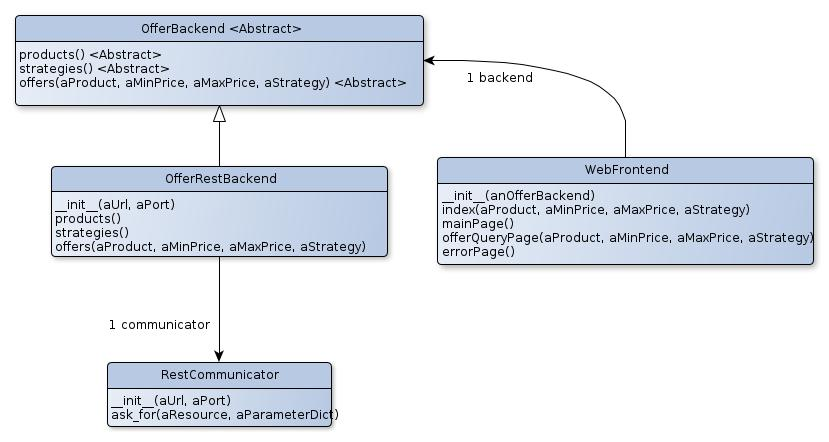
\includegraphics[scale=0.6]{graphics/frontend_class.jpg}
\caption{Frontend}
\end{figure}

linea1\\
linea2\\
\begin{figure}[H]
\centering
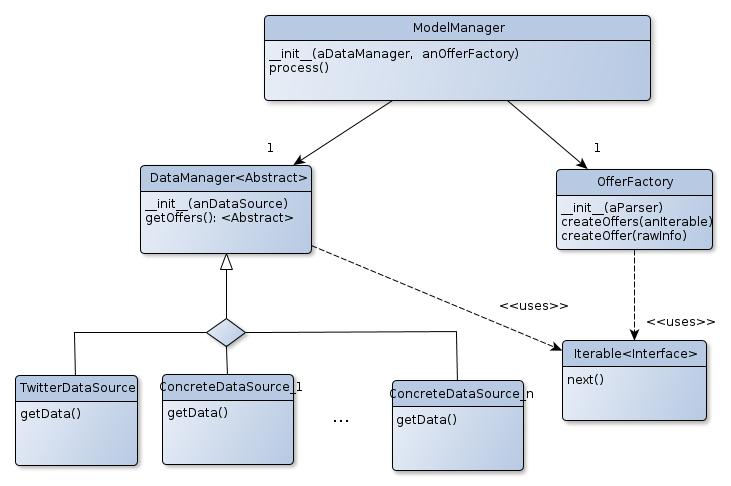
\includegraphics[scale=0.55]{graphics/model_manager_iterable_class.jpg}
\caption{Model Manager Iterable}
\end{figure}

\newpage
linea1\\
linea2\\
\begin{figure}[H]
\centering
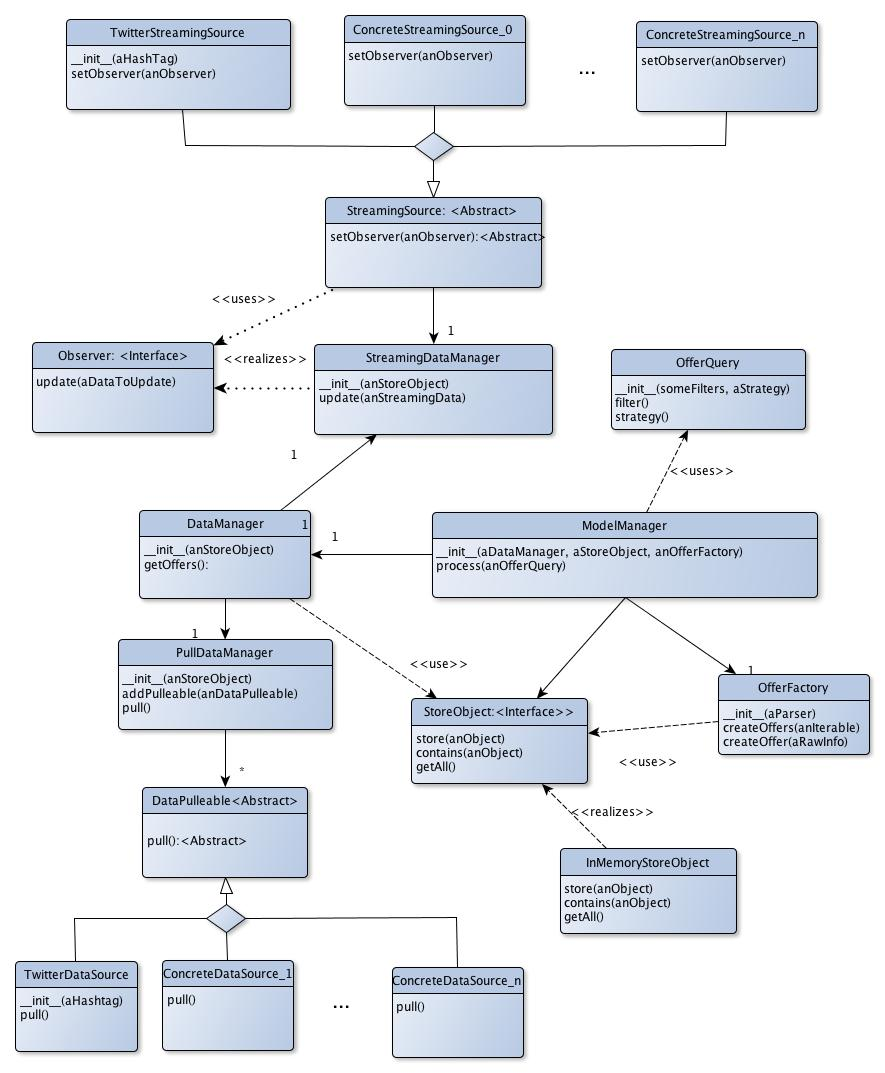
\includegraphics[scale=0.6]{graphics/model_manager_storeObject_class.jpg}
\caption{Model Manager StoreObject}
\end{figure}

\newpage
Para pasar de los Twits (u otro medio, ya que en este punto es transparente el origen de la información) a ofertas entendibles en nuestro sistema. Implementamos un \textbf{OfferFactory} el cual es capas de tranformar una lista de twits (validos o no) en una lista de offertas validas.\\

Para esto el OfferFactory es inicializado con un \textbf{ParserChain} que se encarga de intentar parsear la informacion de los twits devolviendo como resultado un \textbf{OfferBuilder} o la excepcion  \textbf{ParserError} en caso de no ser posible para el parser extrar la informacion para rellenar el OfferBuilder.\\

El ParserChain es Inicializado con una lista de \textbf{SpecificParser}, los cuales son llamados en el orden en el que vienen en la lista, tratando de extrar la informacion que necesitan y volcandola dentro del OfferBuilder que se esta rellenado.\\

Este diseño nos da una gran flexibilidad para los cambios futuros, tanto en agregar nuevas formas de extraer datos, como tambien alterar la forma en la que se extraen los dados ahora sin modificar otras.\\

Como por ejemplo seria muy facil agregar el validador ortografico para poder detectar productos mal escritos sin necesidad de alterar nunguna otra parte (en el diseño se muestra una clase tentativa que le agrega a \textbf{ProductParser} la posibilidad de chequear esto).\\

Lo mismo se aplica con la posibilidad de agregar validaciones a la \textbf{Location} la cual por el momento solo consiste en un string que no tiene ningun tipo de chequeo sobre su validez.\\



\begin{figure}[H]
\centering
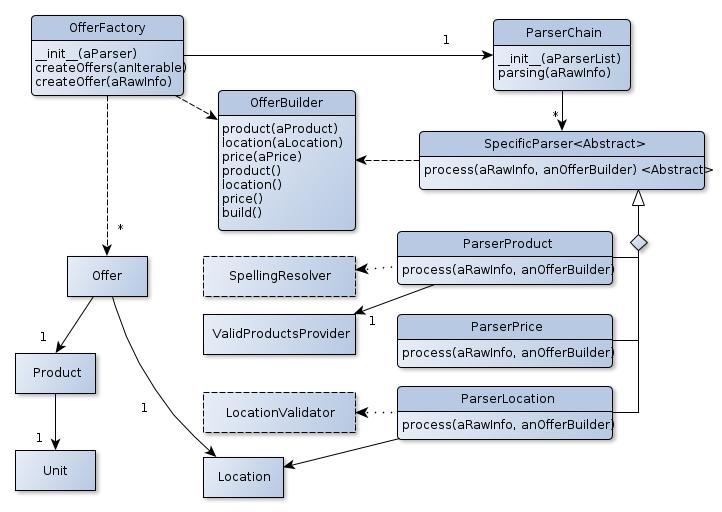
\includegraphics[scale=0.65]{graphics/parser_class.jpg}
\caption{Offer Factory}
\end{figure}
\begin{landscape}

\newpage
linea1\\
linea2\\
\begin{figure}[H]
\centering
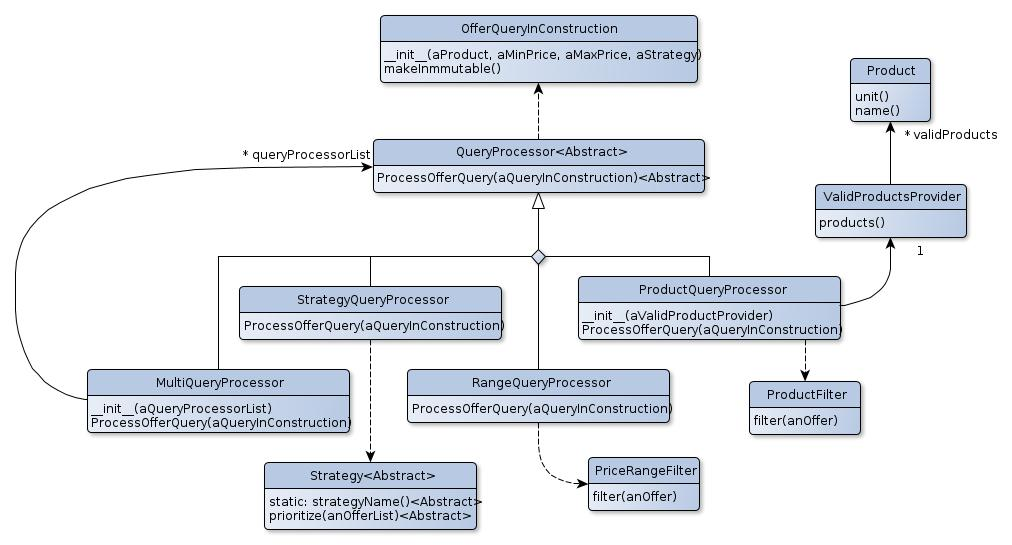
\includegraphics[scale=0.65]{graphics/queryProcessor_class.jpg}
\caption{Query Processor}
\end{figure}

\newpage
linea1\\
linea2\\
\begin{figure}[H]
\centering
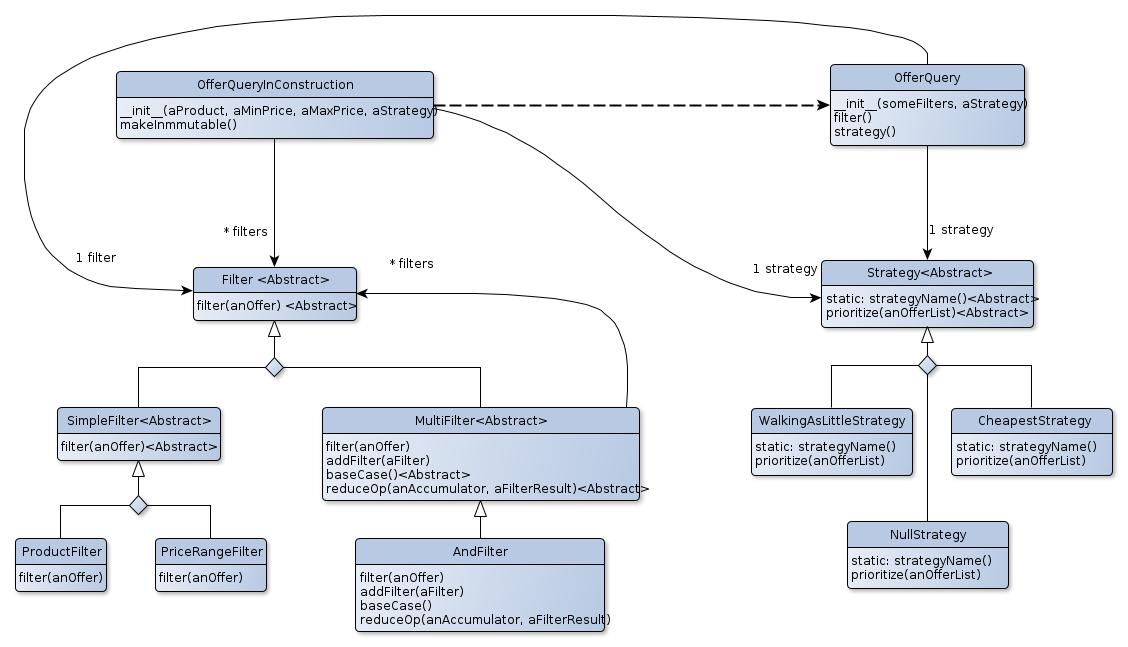
\includegraphics[scale=0.65]{graphics/filter_class.jpg}
\caption{Filter}
\end{figure}



\newpage
\subsection{Diagramas de secuencias}
linea1\\
linea2\\
\begin{figure}[H]
\centering
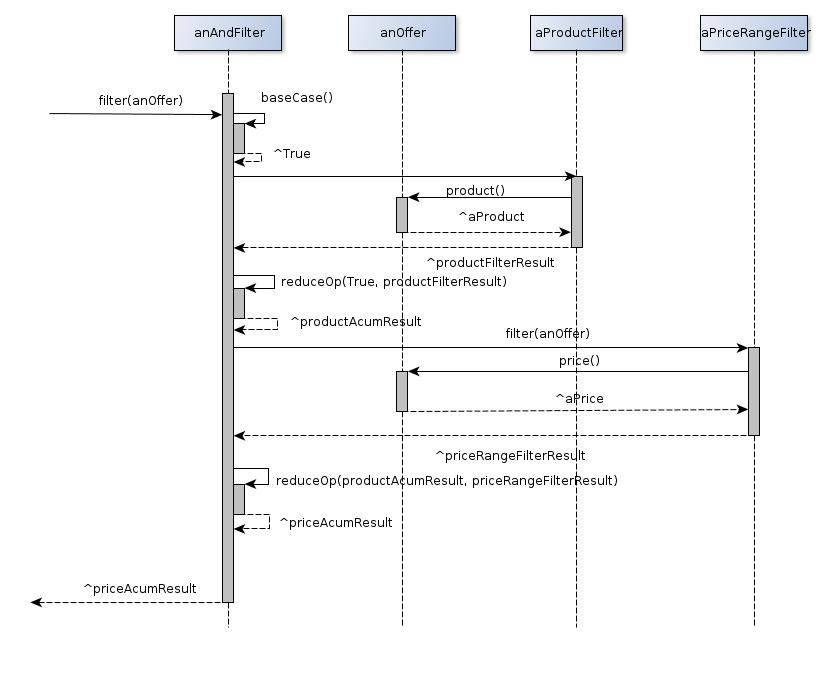
\includegraphics[scale=0.6]{graphics/andFilter_sequence.jpg}
\caption{andFilter}
\end{figure}
\newpage
linea1\\
linea2\\
\begin{figure}[H]
\centering
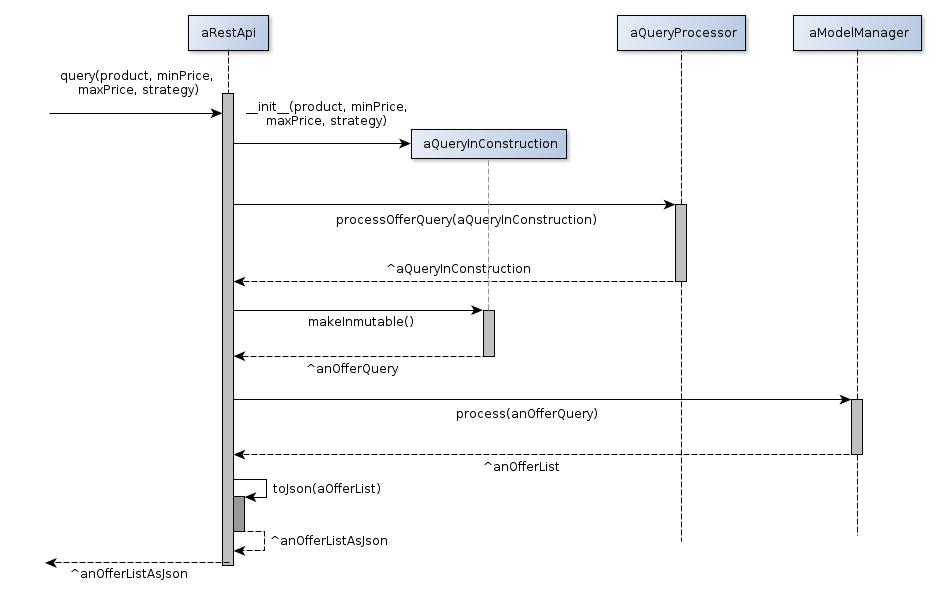
\includegraphics[scale=0.70]{graphics/service_sequence.jpg}
\caption{Service}
\end{figure}
\newpage
linea1\\
linea2\\
\begin{figure}[H]
\centering
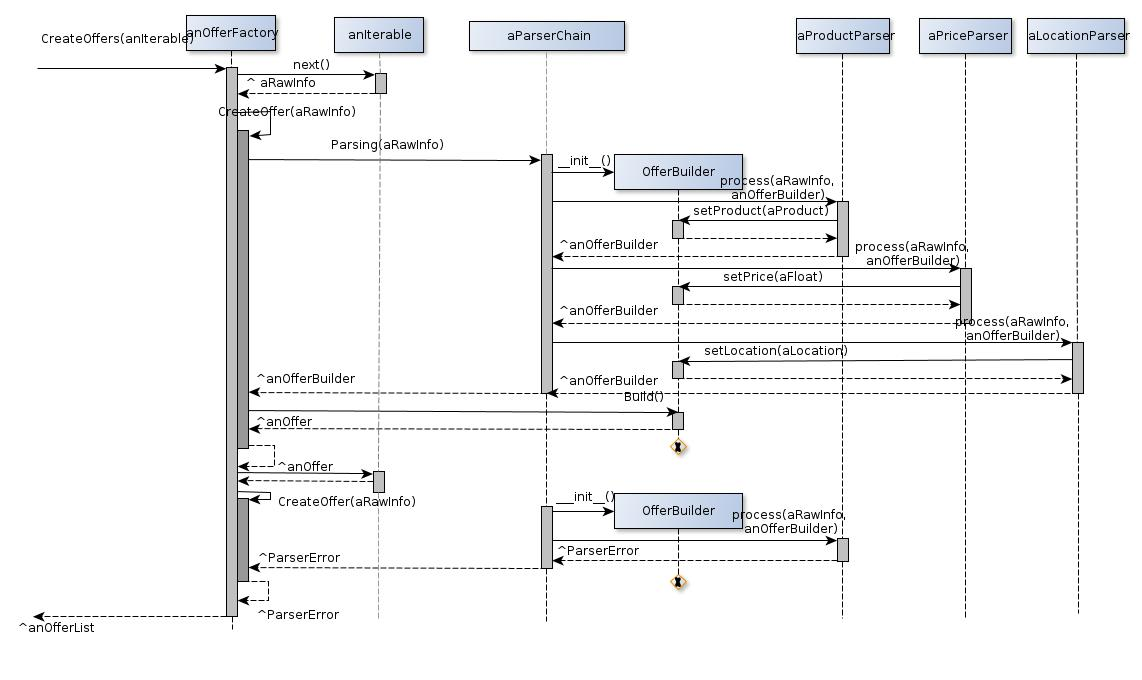
\includegraphics[scale=0.60]{graphics/OfferFactory_sequence.jpg}
\caption{Offer Factory}
\end{figure}

\end{landscape}

\section{Primera Iteración}

En un esquema de desarrollo iterativo incremental, el producto final se construye en iteraciones. En cada iteración se establecen ciertos objetivos, que apuntan a agregar una nueva funcionaliad al producto. Para el momento de este informe, se desarrolló solo la primera iteración. En la misma, el objetivo definido fue tener una primera versión de la aplicación con una funcionalidad limitada, pero completa frente al espíritu del proyecto. El resultado de una iteración se denomina \emph{product increment}. En el \emph{product increment} se deberá permitir buscar las ofertas de un producto en \emph{twitter}, filtrarlos con algún criterio y priorizalos mediante alguna estrategia.

A continuación explicamos como resulto el desarrollo de la primera iteración.

\subsection{Desarrollo}

En el ámbito del trabajo que se está realizando, es importante remarcar el hecho que el desarrollo iterativo incremental de la aplicación fue en el marco de un trabajo práctico cuyos objetivos exceden (en incluso son conflictivos con) los objetivos normales de una iteración. 

\begin{figure}[H]
\centering
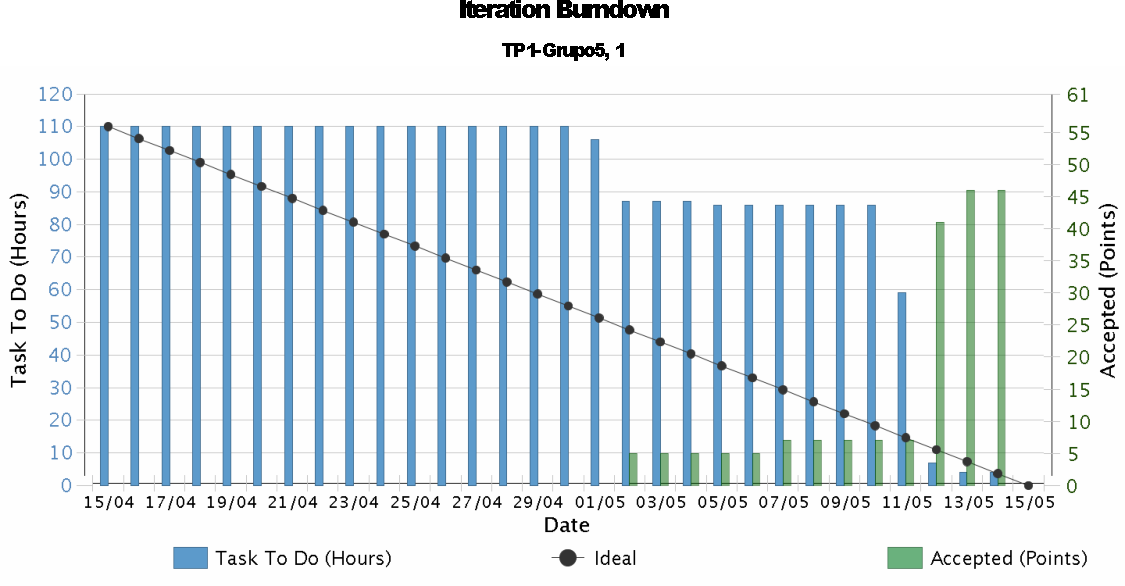
\includegraphics[scale=1.2]{graphics/iteration_burndown.pdf}
\caption{\textbf{Burndown chart:} progreso de terminación de tareas en el \emph{sprint}.}
\end{figure}

\subsection{Logros}

\subsection{Review}

\end{document}
